\chapter{Design}
\label{cha:Design}

\section{S2S}{}
\label{sec:S2S}
The S2S merge is the simplest of those described in Chapter \ref{cha:Problem Analysis}. Any merging system must perform well in the S2S merge before being developed further to tackle more complex merge problems.

\subsection{User controls}
\label{subsec:User controls}
Users of the simulator should be able to adjust simulation features in order to test how different factors affect the performance of the system.

\begin{itemize}
\item \textit{Traffic Level}
Dictates the rate at which vehicles spawn. The higher the traffic level, the greater the spawn rate of each lane.
\item \textit{Target lane speed limit}
The maximum speed that vehicles on the target lane can travel.
\item \textit{Merge lane speed limit}
The maximum speed that vehicles on the merge lane can travel.
\item \textit{Target lane lead in distance}
The distance between the target vehicle spawn point and the point at which the target lane and merge lane end.
\item \textit{Target lane lead out distance}
The distance between where a target vehicle leaves the map and the end of the area where the target lane and merge lane meet.
\item \textit{Merge lane lead in distance}
The distance between where a merge vehicle spawns and where the target lane meets the merge lane.
\item \textit{Merging Angle}
The interior angle $\theta$ at the point where the merging lane meets the target lane.
\end{itemize}

Figure \ref{fig:s2sMarked} illustrates some of the user controllable parameters.

\begin{figure}[htb]
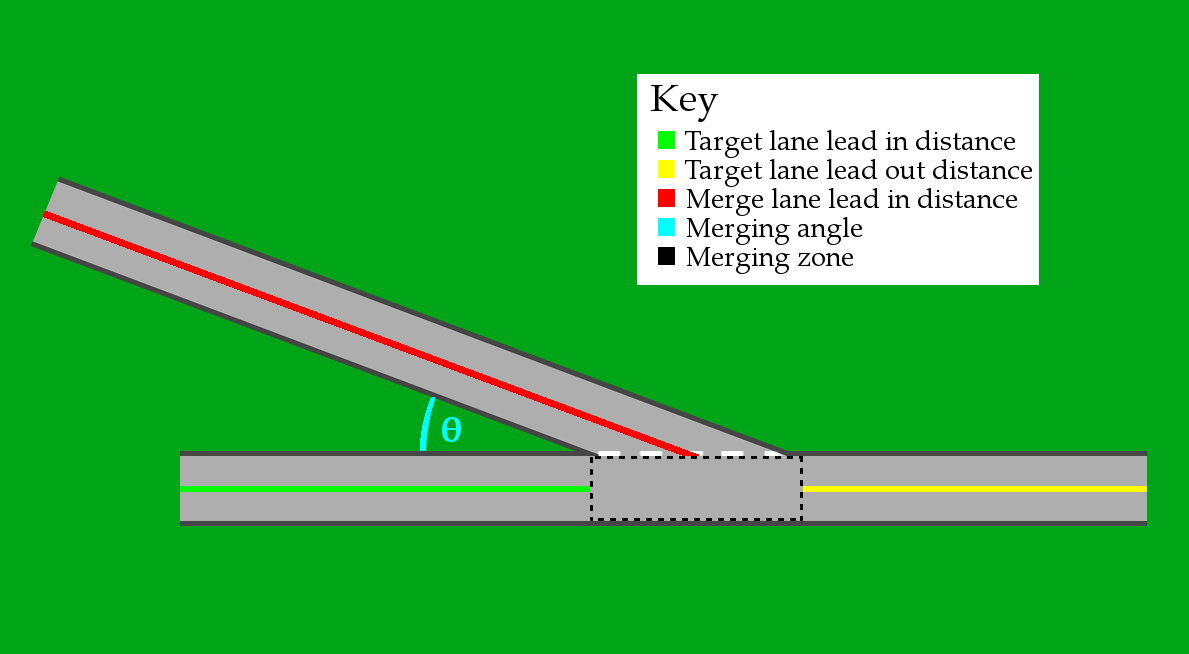
\includegraphics[width=\textwidth]{designNotes/s2sMarked.png}
\caption{An S2S diagram marked with some of the user controllable parameters.}
\label{fig:s2sMarked}
\end{figure}

\subsection{Map}
\label{subsec:Map}
In order to build the map using the user's parameters we will need to calculate the relative positions of the lane entrances and exits as well as the locations of the data collection lines and spawn points.

To start with, we need to calculate the dimensions of the merging zone. The height of the merging zone will be the same as lane width of the target lane. The length can be calculated using the right-angled triangle in Figure \ref{fig:mergingZoneTriangle}. Using this triangle and some trigonometry we can calculate the length of the merge zone ($h$ in Fig. \ref{fig:mergingZoneTriangle}) using equation \ref{hSin}.

\begin{figure}[htb]
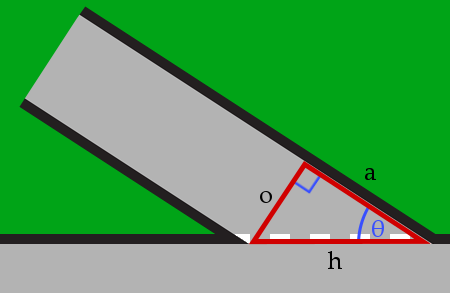
\includegraphics[width=\textwidth]{designNotes/mergingZoneTriangle.png}
\caption{A right-angled triangle used to calculate the size of the merging zone.}
\label{fig:mergingZoneTriangle}
\end{figure}

\begin{equation}\label{hSin}
h = o / \sin(\theta)
\end{equation}

We also need to know whether the horizontal width of the merge lane on the map, or it's 'base width' is longer than the target lane's lead in distance, plus the merge zone length. This will determine the width of the overall map, as if the merge lane's base length is longer then the target lane will not start with co-ordinate $x=0$ as it would if the target lane determined the width of the map.

Firstly we need to calculate the X and Y adjustments at the merge lane entrance. Because the vehicles drive in the centre of the lane and the merge lead in distance is defined by the middle line of the lane we still need to calculate how far the lane extends in the x and y directions due to it's width. To do this we can use the right-angled triangles shown in Figure \ref{fig:mergeEntranceTriangles}

\begin{figure}[htb]
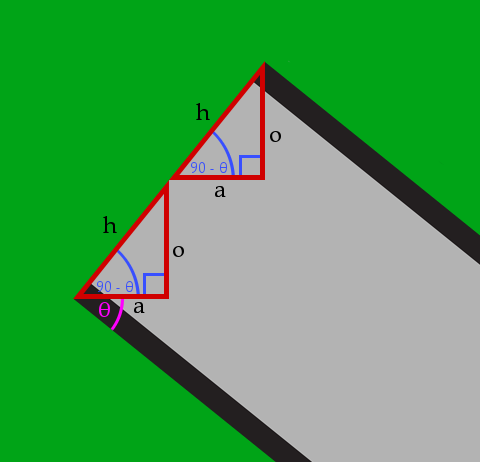
\includegraphics[width=\textwidth]{designNotes/mergeEntranceTriangles.png}
\caption{Two right-angled triangles used to calculate the x and y adjustments for the merge entrance.}
\label{fig:mergeEntranceTriangles}
\end{figure}

These triangles have the same dimensions and have an interior angle of 90 - $\theta$ due to the 'alternate angle' or 'z-angle' rule. Each triangle has a hypotenuse with a length equal to half the width of the lane. 

The x-adjustment for the merge entrance is the length of the adjacent side of one of the lower triangle and the y-adjustment for the merge entrance is the length of the opposite side of the upper triangle (though both triangles do have the same dimensions). We can use equation \ref{aCos90} to calculate the X-adjustment and equation \ref{oSin90} to calculate the Y-adjustment.

\begin{equation}\label{aCos90}
a = h \cos(90 - \theta)
\end{equation}{}

\begin{equation}\label{oSin90}
o = h \sin(90 - \theta)
\end{equation}

To calculate the 'base width' of the merge lane we will also need to calculate the adjacent side of the triangle in Figure \ref{fig:baseWidthTriangle}. In this triangle the hypotenuse has a length equal to the merge lead in distance. Therefore, we can use equation \ref{aCos} to calculate the length of the adjacent side. After obtaining the length of this side we simply add the merge entrance X-adjustment and half the length of the merge zone to find the merge base width.

\begin{figure}[htb]
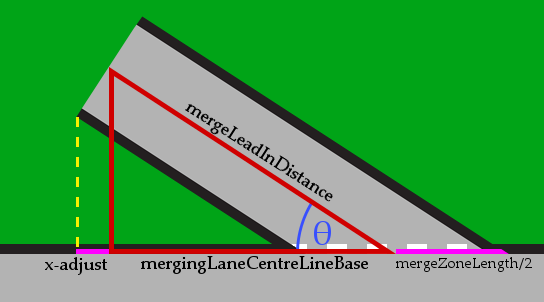
\includegraphics[width=\textwidth]{designNotes/baseWidthTriangle.png}
\caption{A right-angled triangle used to help calculate the base width of the merge lane, along with the X-adjustment and merge-zone length.}
\label{fig:baseWidthTriangle}
\end{figure}

\begin{equation}\label{aCos}
a = h \cos(\theta)
\end{equation}

We also need to find the point at which the merging lane's centre line crosses the target lane's centre line in the merge zone. We know the Y-coordinate for this point as it will be the same as the Y-coordinate of the target lane centre line. We also know the X-coordinate of the point at which the merge lane's centre line meets the target lane. We can use these two co-ordinates to create the triangle shown in Figure \ref{fig:toCentreTriangle}. We can then use equation \ref{aTan} to find the X-adjustment from the merge zone centre to the point where the two centre lines cross.

\begin{figure}[htb]
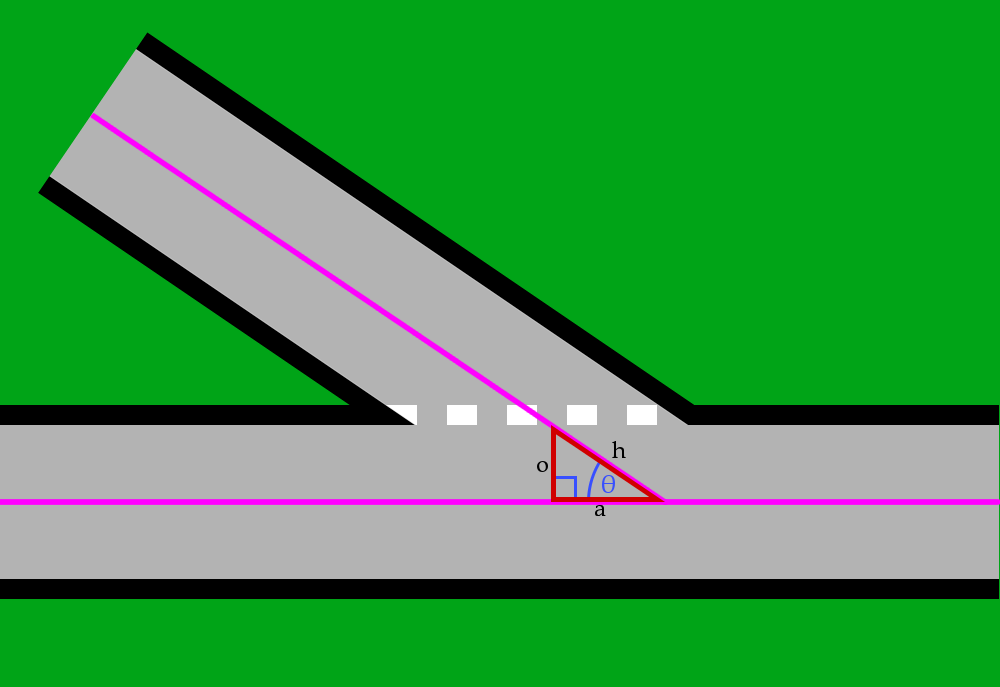
\includegraphics[width=\textwidth]{designNotes/toCentreTriangle.png}
\caption{A right-angled triangle used to calculate where the two centre lines meet. The centre lines are indicated in pink.}
\label{fig:toCentreTriangle}
\end{figure}

\begin{equation}\label{aTan}
a = o / \tan(\theta)
\end{equation}

\subsection{Intersection Management System}
\label{subsec:Intersection Management System}

\subsection{Decentralised Communication System}
\label{subsec:Decentralised Communication System}

\subsection{Measuring Success}
\label{subsec:Measuring Success}
